\chapter{Data sources}
\label{app:data-sources}

There are various sources of relevant data in terms of my research and research into mobile analytics necessarily includes the data and reports that are made available through mobile analytics. These data and reports are primarily aimed at the development teams responsible for the respective mobile apps. Other data sources include source code and bug tracking systems. 

Various development teams made at least some of their mobile analytics reports, data, source code, and/or bug tracking systems available for research purposes. Some provided occasional snapshots, others access for a period, and some provided access on a long term basis.

\section{Characterising the data as presented}
The providers of the analytics services choose and constrain what data is available, to whom, and for how long. App, developer, and organisation specific mobile analytics are private and only available to authorised users of the respective services and accounts.

The analytics services present their data in at least one form, the most common being via web pages that include visual reports. The others include: file downloads, API access, proprietary mobile apps, and vendor specific exports to one or more cloud-hosted services. Some also provide integration with issue/bug management tools.

Examples of web pages include the two shown in Figure~\ref{fig:examples-of-sentry-io-mobile-analytics-reports} from \href{https://sentry.io/}{sentry.io} which show the ranked set of recent issues detected by \href{https://sentry.io/}{sentry.io} for the LocalHalo app, and the two shown in Figure~\ref{fig:examples-of-gpc-with-av-mobile-analytics-reports} from Google Play Console for the main Kiwix Android app. 

\begin{figure}
    \centering
    \subfloat[Issues Report]{{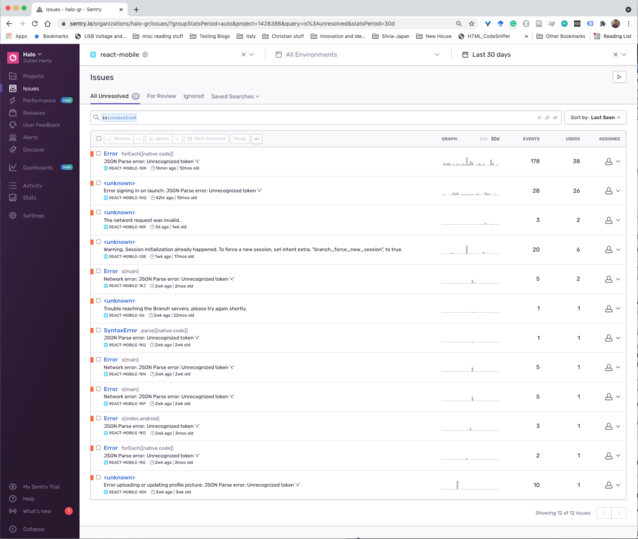
\includegraphics[width=6cm]{images/sentry.io/sentry.io-issues-page-resized.png} }}
    \qquad
    \subfloat[Individual Error Details]{{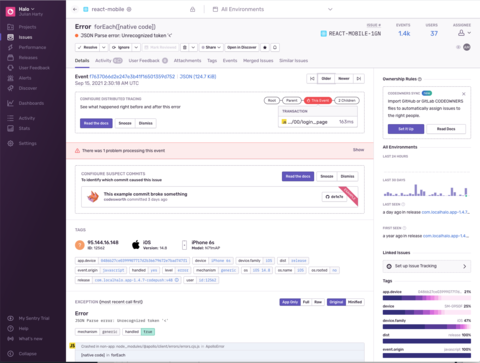
\includegraphics[width=6cm]{images/sentry.io/sentry.io-error-page-resized.png} }}
    \caption{Examples of sentry.io mobile analytics}
    \label{fig:examples-of-sentry-io-mobile-analytics-reports}
\end{figure}

\begin{figure}
    \centering
    \subfloat[Dashboard for Kiwix]{{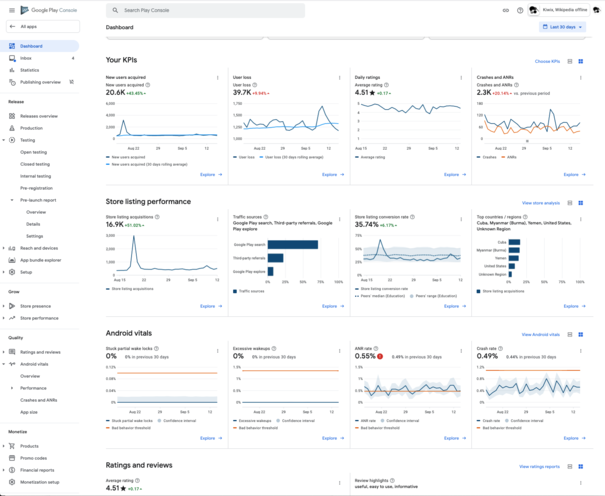
\includegraphics[width=6cm]{images/android-vitals-screenshots/kwix/resized-example-for-kiwix-dashboard-2021-sep-16.png} }}
    \qquad
    \subfloat[ANR's for Kiwix in Android Vitals]{{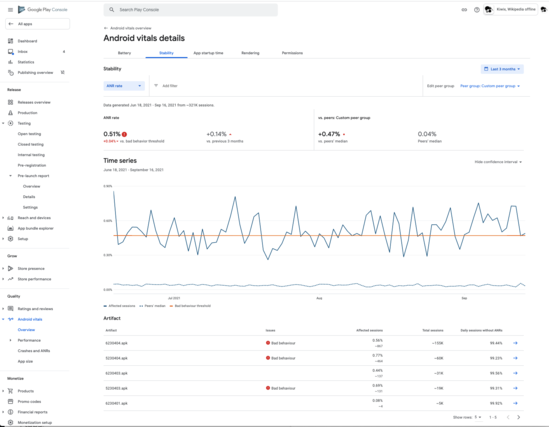
\includegraphics[width=6cm]{images/android-vitals-screenshots/kwix/resized-example-of-android-viatals-anr-chart-2021-sep-16.png} }}
    \caption{Examples of Google Play Console mobile analytics}
    \label{fig:examples-of-gpc-with-av-mobile-analytics-reports}
\end{figure}
% Thanks to https://resizeimage.net/ for enabling easy resizing of the screenshots and 
%  https://www.codegrepper.com/code-examples/whatever/how+to+set+two+images+side+by+side+in+latex for the above latex.

When the data is presented visually (as web pages or in mobile apps) many of the reports are interactive, and some can be customised to varying degrees. The contents are often dynamic and recent, and therefore ephemeral. While reports these are useful for developers they do not necessarily facilitate further processing, storage, or analysis of the underlying data. Web scraping is one approach to extracting data from web pages; \href{section-vitals-scraper}{\nameref{section-vitals-scraper}} was developed as part of this research to preserve reports and data from Google Play Console with Android Vitals. The challenges, design, and implementation are discussed in that section of this thesis. In terms of this topic, data sources, Vitals Scraper enabled copies of visual reports in Google Play Console to be preserved as PDF files, summary data to be exported as a CSV file. It also exported and crash and ANR clusters were exported from Android Vitals in the JSON format.

Interactive downloads reduce the need to parse web pages that contain the same underlying data and therefore a mechanism to improve the working life of the data, however in practice often they contain a small subset of the data. They are also a static snapshot, \textit{i.e.} they are not updated by the provider once they have been downloaded. A germane example of one of the extracts available from a visual report in Android Vitals is illustrated in Listing~\ref{listing:crash-stack-trace-in-kiwix}. This facility was added to Android Vitals in 2021 and a good example of how providers change the capabilities and features of their mobile analytics from time to time.

Google Play Console also provides various downloadable daily summary reports. The details change from time to time, the current details should be available online at \url{https://support.google.com/googleplay/android-developer/answer/6135870}.

{\footnotesize
\begin{quote}
    `Control access to Google Cloud Storage
    Reports available on Google Cloud Storage use the same access restrictions that control data access on your Play Console. This means account users with access to areas of a Play Console account have access to the corresponding reports in Google Cloud Storage.
    
    Account owners can update permissions for individual users at any time.
    
        To access bulk reports, your "View app information" permission must be set to "Global."
        To download financial reports, your "View financial data" permission must be set to "Global." '
\end{quote}}~\citep{google_play_download_and_export_monthly_reports}~\footnote{in 2020, this help page  \url{https://support.google.com/googleplay/android-developer/answer/6135870} stated the developer's user account needed to be given 'Global' permission rather than per-app. In 2021 the same article no longer explains what permissions are needed, however another help page \url{https://support.google.com/googleplay/android-developer/answer/9844686} partly answers the permissions that needs to be granted.}

Here are the instructions for how to change the setting to Global \url{https://support.google.com/googleplay/android-developer/answer/2528691}

Where and when the data is available using APIs and/or available for ongoing cloud-based processing there is the greatest flexibility and opportunity for development teams (and others with access) to perform ad-hoc and ongoing analysis. When providers do offer these services, they sometimes need to be paid for on an ongoing basis. 

\begin{lstlisting}[language=json, caption=Exported contents for a crash reported in Android Vitals in Sept 2021, label=listing:crash-stack-trace-in-kiwix]
  java.lang.IllegalStateException: 
  at androidx.fragment.app.Fragment.requireContext (Fragment.java:805)
  at androidx.fragment.app.Fragment.getResources (Fragment.java:869)
  at androidx.fragment.app.Fragment.getString (Fragment.java:891)
  at org.kiwix.kiwixmobile.core.main.CoreReaderFragment.webViewFailedLoading (CoreReaderFragment.java:1478)
  at org.kiwix.kiwixmobile.core.main.CoreWebViewClient.onReceivedError (CoreWebViewClient.java:112)
  at android.webkit.WebViewClient.onReceivedError (WebViewClient.java:298)
  at fz.handleMessage (chromium-Monochrome.aab-stable-457706223:125)
  at android.os.Handler.dispatchMessage (Handler.java:109)
  at android.os.Looper.loop (Looper.java:166)
  at android.app.ActivityThread.main (ActivityThread.java:7555)
  at java.lang.reflect.Method.invoke (Native Method)
  at com.android.internal.os.RuntimeInit$MethodAndArgsCaller.run (RuntimeInit.java:469)
  at com.android.internal.os.ZygoteInit.main (ZygoteInit.java:963)
\end{lstlisting}

\section{Google Play}
Google Play provides a public end-user orientated visual view of apps in Google Play. It also provides a developer-oriented view of \emph{their} apps\footnote{More correctly, apps they are permitted to view and manage. Google provides account owners the ability to invite people to view, and potentially manage, one or more Android apps. Not everyone who has access is a developer, nonetheless the reports, tools, etc. are aimed primarily for developers.}; this is known as Google Play Console.

\section{Google Play Console}
Monthly reports are available for developers to download, they include: Install statistics, Crash statistics, Rating statistics, Reviews and Retained installers. 

Google provides several online help pages on the monthly reports~\citep{google_play_download_and_export_monthly_reports}. They do not describe the fields or the character encoding of the contents of the files. The files start with a two-character code \texttt{0xFE 0xFF} which indicate the contents of the file is encoded as UTF-16 little-endian. These seemingly useful characters can prevent the content from being loaded in many programs and utilities intended to work with CSV data.

\subsection{Defunct reports}
Various reports used to be available to download, Google chose to remove them~\citep{google_play_download_and_export_monthly_reports}. The removed reports include: subscription acquisition (removed November 2019), detailed crash and detailed ANR reports (removed May 2018).

\subsection{Coping with UTF-16 content}
Google provides the files encoded in UTF-16 format. The default import tool in the R programming language fails to import data in this (or many other encodings). Through research and experiments the following code snippet is able to load downloaded crash reports into a Data Frame in R.

\begin{lstlisting}[language=R, caption=Processing UTF-16 contents using R, label=listing=processing-utf-16-contents-in-r]
  setwd("\textbf{$_{\widetilde{~}}$}")  %All this to display a tilde adequately.
  filenames = list.files("./Dropbox/Google Play Console Reports/reports/kiwix/", pattern = ".csv")
  directory = "./Dropbox/Google Play Console Reports/reports/kiwix/"
  filenames <- paste(directory, filenames, sep="/")
  CrashAndAnrStats <- lapply(filenames, read.csv, fileEncoding="UTF-16")
\end{lstlisting}

Data I downloaded (not necessarily used) include reviews stored in Google Drive.

\subsection{Obtaining the data}
Google provide two documented ways to obtain the reports. The simplest for occasional use is to download the reports from the relevant \emph{Download Reports} section in Google Play Console. The second is to configure and use the \texttt{gsutil} command-line tool.

\subsubsection{Interactive per-file downloads}
The interactive GUI for download reports leads to three menu options: Reviews, Statistics, and User acquisition. Statistics includes three types of information: Install statistics, Rating statistics, and Crash statistics. The other two menu options offer a single type of information: \emph{Reviews}, and \emph{Retained installers} for user acquisition.

\subsubsection{gsutil}
Google provides a command-line tool called \emph{gsutil}\footnote{Perhaps the name is based on \underline{G}oogle \underline{S}torage \underline{util}?} which can be used to download reports in bulk. While Google encourages people to create and configure a Google Cloud account and use gsutil from the Google Cloud sdk, they also provide the file as a separate download together with installation~\footnote{Installation instructions for gsutil \url{https://cloud.google.com/storage/docs/gsutil_install}} and configuration instructions~\footnote{\url{https://cloud.google.com/storage/docs/gsutil_install\#creds-gsutil}}. I chose to use the standalone version of gsutil and was able to install and configure it without problems.  

Example command-lines are provided in the documentation, these need to be edited to point to the correct project bucket for a given app's data, and similarly unless all the files are to be downloaded, a suitable wildcard provided for gsutil.  
% https://cloud.google.com/storage/docs/quickstart-gsutil

%%%% Example command-lines
% gsutil -m cp -r gs://pubsite_prod_rev_14876298819229479527/stats/crashes/crashes_org.kiwix.kiwixcustomphet_20* .
% gsutil -m cp -r gs://pubsite_prod_rev_14876298819229479527/stats/installs/installs_org.kiwix.kiwixcustomphet_20* .

\subsection{Installs}
Installs are important as one measure of success of an app. Mainstream Android apps need to be installed before they can be used (unlike web apps, for instance which are not explicitly 'installed'). 

\subsubsection{Assumptions for Installations } 
One assumption is that new apps should start with no installs, the second is that there are more installs than uninstalls, in other words the total number of uninstalls cannot exceed the total number of installs (assuming they are measured and counted similarly).

Analysing Installs: 
\begin{enumerate}
    \item Obtain data from Google Play
    \item Gather data from files into linear list, coping with changes in file structure over time.
    \item Interpret fields as best possible.
    \item Estimate which fields are correctly populated.
    \item Generate equivalent reports to those presented in Google Play Console.
\end{enumerate}

\subsubsection{Fields change over time in files}
We observed several changes in the contents of the monthly files with three different formats in the first six months of the installs files for the Chemistry and Physics Simulations Kiwix app. These changes made the data harder to compare and analyse as several fields are not consistently available over the history of the data.
% (a) Date,Package Name,Current Device Installs,Daily Device Installs,Daily Device Uninstalls,Daily Device Upgrades,Current User Installs,Total User Installs,Daily User Installs,Daily User Uninstalls
% (b) Date,Package Name,Current Device Installs,Daily Device Installs,Daily Device Uninstalls,Daily Device Upgrades,Current User Installs,Total User Installs,Daily User Installs,Daily User Uninstalls,Active Device Installs
% (c) Date,Package Name,Daily Device Installs,Daily Device Uninstalls,Daily Device Upgrades,Total User Installs,Daily User Installs,Daily User Uninstalls,Active Device Installs
\begin{table}[htbp!]
    \centering
    \footnotesize
    \begin{tabular}{lll}
    (a) &(b) &(c)\\
    \hline
    Date &Date &Date\\
    Package Name &Package Name &Package Name\\
    Current Device Installs &Current Device Installs &\\
    Daily Device Installs &Daily Device Installs &Daily Device Installs\\
    Daily Device Uninstalls &Daily Device Uninstalls &Daily Device Uninstalls\\
    Daily Device Upgrades &Daily Device Upgrades &Daily Device Upgrades\\
    Current User Installs &Current User Installs &\\
    Total User Installs &Total User Installs &Total User Installs\\
    Daily User Installs &Daily User Installs &Daily User Installs\\
    Daily User Uninstalls &Daily User Uninstalls &Daily User Uninstalls\\
                          &Active Device Installs &Active Device Installs\\
    \end{tabular}
    \caption{File Formats for Installs}
    \label{tab:file_formats_for_installs}
\end{table}

The changes in the columns means that more work is needed to combine the data consistently for reporting and analysis. 

\begin{lstlisting}[language=R, caption=Code snippet in R showing the error reported when columns in the data to import do not match, label=listing:r-import-error-code-snippet]
installs_data <- do.call(rbind, installs)
Error in rbind(deparse.level, ...) : 
  numbers of columns of arguments do not match
\end{lstlisting}

An article by Amy Whitehead~\footnote{\url{https://amywhiteheadresearch.wordpress.com/2013/05/13/combining-dataframes-when-the-columns-dont-match/}}, together with comments to that article \emph{e.g.} on using \texttt{Reduce()} enabled the data to be loaded despite differences in the columns.
% Also interesting ideas in https://stackoverflow.com/questions/26874710/how-does-one-combine-two-uneven-dataframes-to-create-a-full-species-matrix-for-a/26900774#26900774

\subsubsection{Processing Dates}
The source data files have the date as the first column in \texttt{YYYY-MM-DD} format. When these were loaded into R using \texttt{read.csv} the dates were converted into vectors. The dates are hard to process or analyse as vectors. 

The first approach was to use \texttt{flipDate} an opensource R package~\cite{r_date_conversion_github}, documentation is available in an online article~\cite{r_date_conversion_article}. \texttt{flipDate} is able to convert the dates stored as vectors into R's Date object. We used the \texttt{ymd()} method to do so.

The first approach was replaced by specifying a column class to the \texttt{read.csv} method~\cite{r_bloggers_using_colclasses}. Doing so improves both performance and utility of the data. It also removed the need to use \texttt{flipDate}.

\subsubsection{Dates in filenames}
The filenames represent monthly reports, as such, their name includes the 4 digit year and the month encoded in two digits, from 01 for January to 12 for December. The following listing provides examples of the first six filenames for installs for the Pocket Code.

\begin{comment}


\begin{lstlisting}[language=R, caption=Querying installs using R, label=listing=using-head-for-installs-in-r]
head(install_filenames)
[1] "installs_org.catrobat.catroid_201308_overview.csv"
[2] "installs_org.catrobat.catroid_201309_overview.csv"
[3] "installs_org.catrobat.catroid_201310_overview.csv"
[4] "installs_org.catrobat.catroid_201311_overview.csv"
[5] "installs_org.catrobat.catroid_201312_overview.csv"
[6] "installs_org.catrobat.catroid_201401_overview.csv"
\end{lstlisting}

\end{comment}

%%%% Useful articles include:
% https://stackoverflow.com/questions/17496358/r-help-converting-factor-to-date
% https://www.displayr.com/r-date-conversion/ (mentioned above)
% https://stackoverflow.com/questions/32854538/converting-a-character-string-into-a-date-in-r
% https://www.r-bloggers.com/using-colclasses-to-load-data-more-quickly-in-r/
% https://stackoverflow.com/questions/5158179/processing-date-and-time-data-in-r
% https://www.r-bloggers.com/date-formats-in-r/

The \texttt{Date} datatype enables dates to be analysed and compared \emph{e.g.} \texttt{min("my\_date")}~\cite{r_bloggers_date_formats_in_r}.


\subsection{Crash and ANR Reports}
Google Play Console only provides the Crashes and ANRs in a combined summary report. We created and opensourced \href{https://github.com/commercetest/vitals-scraper}{Vitals Scraper} to enable additional data to be downloaded, including details of crashes and ANR's.

For the summary reports provided by Google Play Console, in \texttt{R} the data was first loaded file by file, each into a distinct \texttt{data.frame}. These are then combined into a single larger data set as follows:  
\texttt{do.call(rbind, crash\_and\_anr\_stats)}\footnote{Using the initial naive approach is enough to obtain the behaviour I sought \url{https://www.r-bloggers.com/concatenating-a-list-of-data-frames/}}

\begin{lstlisting}[language=R, caption=Querying daily crash and ANR statistics files using R, label=listing=using-head-for-crashes-and-anrs-in-r]
head(crash_and_anr_stats[[1]])
        Date         Package.Name Daily.Crashes Daily.ANRs
1 2014-01-02 org.catrobat.catroid             1          0
2 2014-01-04 org.catrobat.catroid             1          0
3 2014-01-05 org.catrobat.catroid             1          0
4 2014-01-11 org.catrobat.catroid             1          0
5 2014-01-12 org.catrobat.catroid             1          0
6 2014-01-14 org.catrobat.catroid             1          0
\end{lstlisting}

We can observe there are dates without data, for instance \nth{3} January 2014 for Pocket Code. One possibility is there were no reported crashes or ANRs for the dates that are not in the reports, Google does not document the contents of the files, so the reason is not known currently.

\section{Fabric Crashlytics}
Fabric Crashlytics and the associated Android programming library and APIs has been used by the Pocket Code Android app for several years, predating my involvement. It was retired by Google in early May 2020, they replaced it with the Firebase Console for the reporting. They also offer a replacement library and APIs which the project has  yet to switch to.

The reports in Fabric and the replacement Firebase console are predominantly graphical and visual in nature. Fabric allowed some of the data in the reports to be exported. Details and examples TBC %MUST_DO continue this section.

\section{Microsoft AppCenter}
We used Microsoft AppCenter with the Zipternet Android app we developed for various reasons, including this research. It is another tool predominantly graphical and interactive in nature.
% MUST_DO extend this section and provide some examples. I need to log back into AppCenter too, I need to remember how I originally logged in though :)

\section{Summary of Data Sources}
My research analysed data using various sources for several case studies. 